%%%%%%%%%%%%%%%%%%%%%%%%%%%%%%%%%%%%%%
%%%%%%%%%%%%%%%%%%%%%%%%%%%%%%%%%%%%%%
% Do not edit the TeX file your work
% will be overwritten.  Edit the RnW
% file instead.
%%%%%%%%%%%%%%%%%%%%%%%%%%%%%%%%%%%%%%
%%%%%%%%%%%%%%%%%%%%%%%%%%%%%%%%%%%%%%




%%%%%%%%%%%%%%%%%%%%%%%%%%%%%
% initial fit for iris
%%%%%%%%%%%%%%%%%%%%%%%%%%%%%
\newcommand{\IrisFit}{

\begin{knitrout}
\definecolor{shadecolor}{rgb}{0.969, 0.969, 0.969}\color{fgcolor}

{\centering 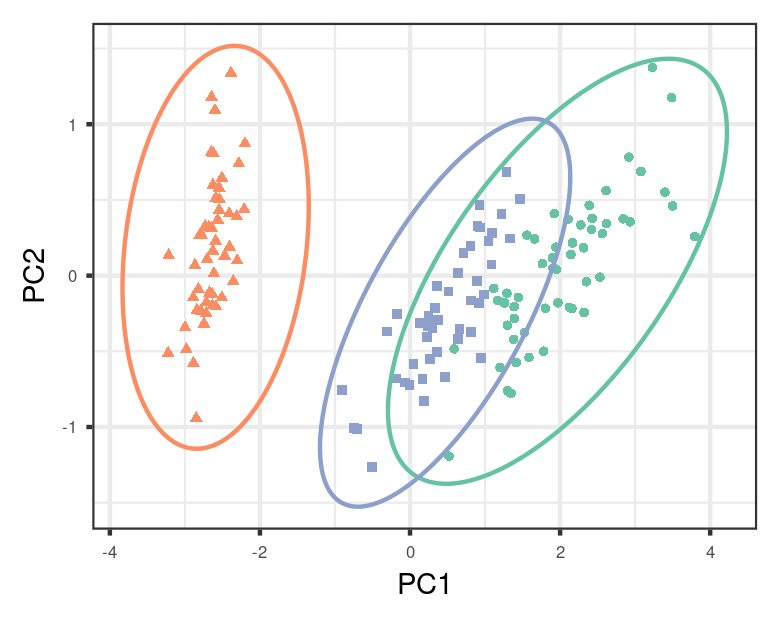
\includegraphics[width=0.637\linewidth,height=0.510\linewidth]{figure/iris_init-1} 

}



\end{knitrout}
}

%%%%%%%%%%%%%%%%%%%%%%%%%%%%%
% iris alpha sensitivity
%%%%%%%%%%%%%%%%%%%%%%%%%%%%%
\newcommand{\IrisAlphaRefit}{


\begin{knitrout}
\definecolor{shadecolor}{rgb}{0.969, 0.969, 0.969}\color{fgcolor}

{\centering 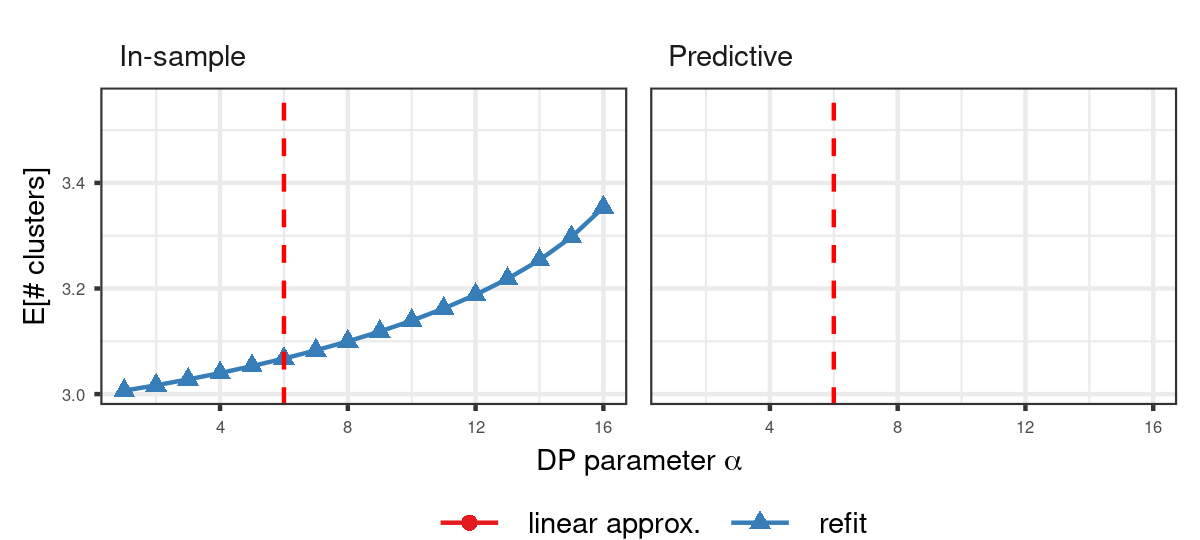
\includegraphics[width=0.980\linewidth,height=0.441\linewidth]{figure/iris_alphasens_refit-1} 

}



\end{knitrout}
}

\newcommand{\IrisAlphaInSample}{
\begin{knitrout}
\definecolor{shadecolor}{rgb}{0.969, 0.969, 0.969}\color{fgcolor}

{\centering 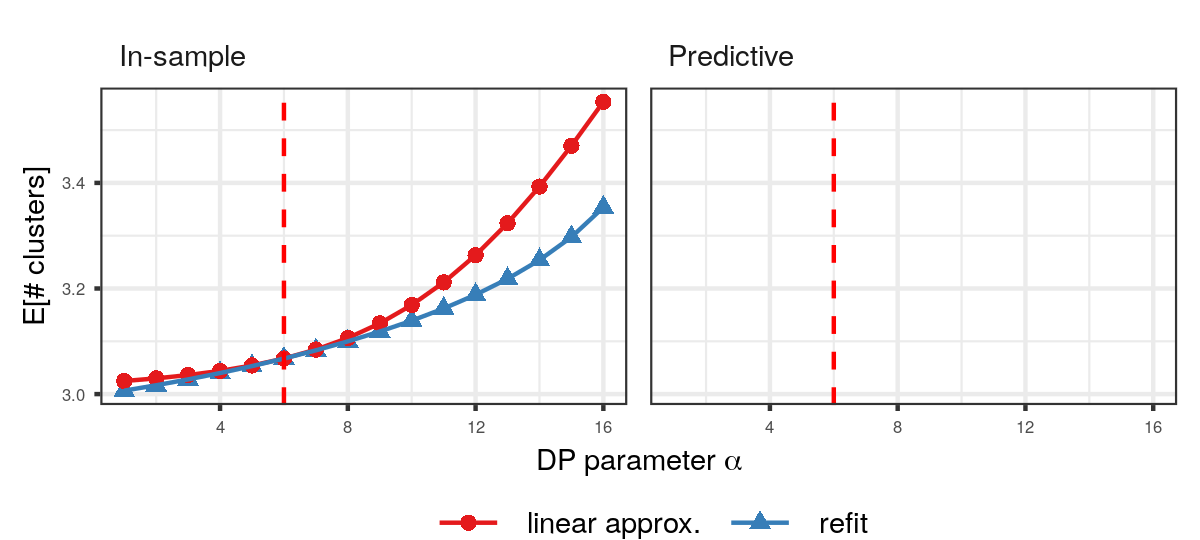
\includegraphics[width=0.980\linewidth,height=0.441\linewidth]{figure/iris_alphasens_insample-1} 

}



\end{knitrout}
}

\newcommand{\IrisAlphaAll}{
\begin{knitrout}
\definecolor{shadecolor}{rgb}{0.969, 0.969, 0.969}\color{fgcolor}

{\centering 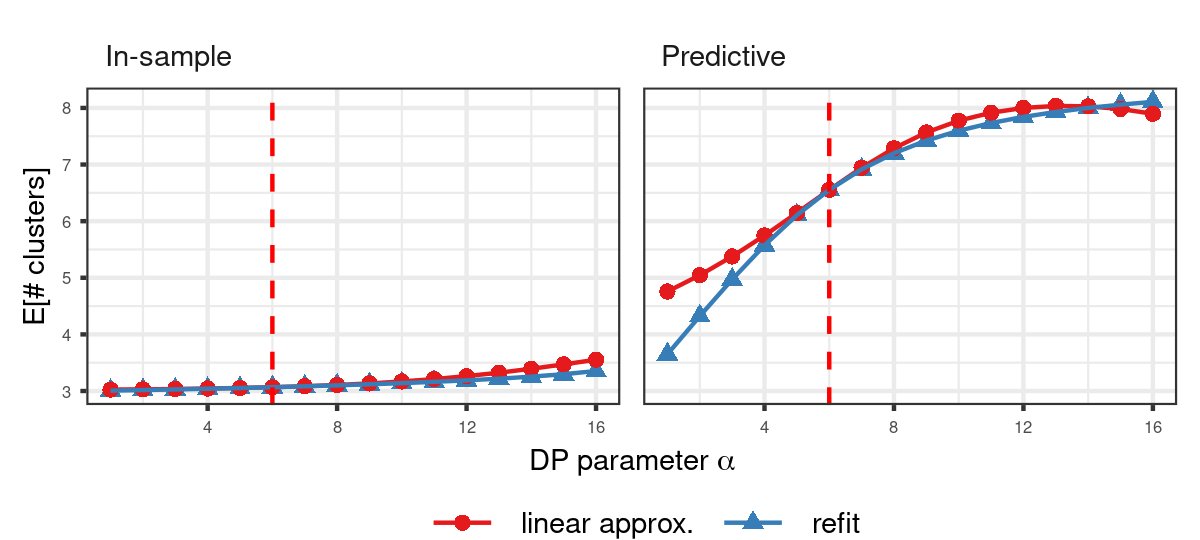
\includegraphics[width=0.980\linewidth,height=0.441\linewidth]{figure/iris_alphasens_all-1} 

}



\end{knitrout}
}


%%%%%%%%%%%%%%%%%%%%%%%%%%%%%
% iris influence function
%%%%%%%%%%%%%%%%%%%%%%%%%%%%%
\newcommand{\IrisInfluence}{

\begin{knitrout}
\definecolor{shadecolor}{rgb}{0.969, 0.969, 0.969}\color{fgcolor}

{\centering 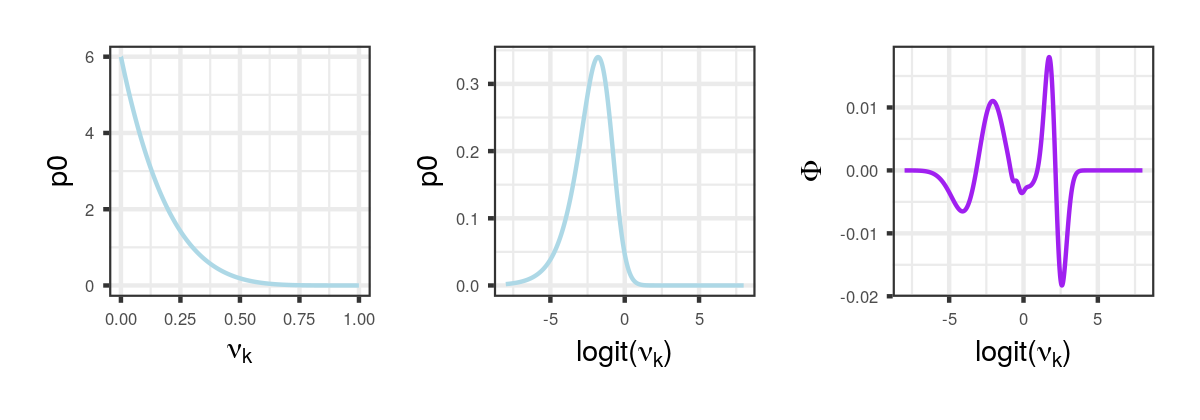
\includegraphics[width=0.980\linewidth,height=0.343\linewidth]{figure/iris_infl-1} 

}



\end{knitrout}
}


%%%%%%%%%%%%%%%%%%%%%%%%%%%%%
% iris function perturbations
%%%%%%%%%%%%%%%%%%%%%%%%%%%%%
\newcommand{\IrisFpertEx}{

\begin{knitrout}
\definecolor{shadecolor}{rgb}{0.969, 0.969, 0.969}\color{fgcolor}

{\centering 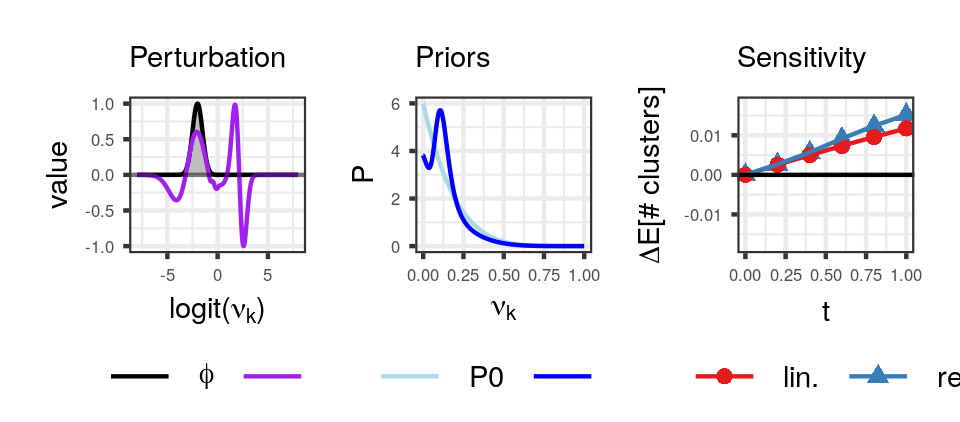
\includegraphics[width=0.784\linewidth,height=0.345\linewidth]{figure/iris_fpertex-1} 

}



\end{knitrout}
}

\newcommand{\IrisFpertAll}{

\begin{knitrout}
\definecolor{shadecolor}{rgb}{0.969, 0.969, 0.969}\color{fgcolor}

{\centering 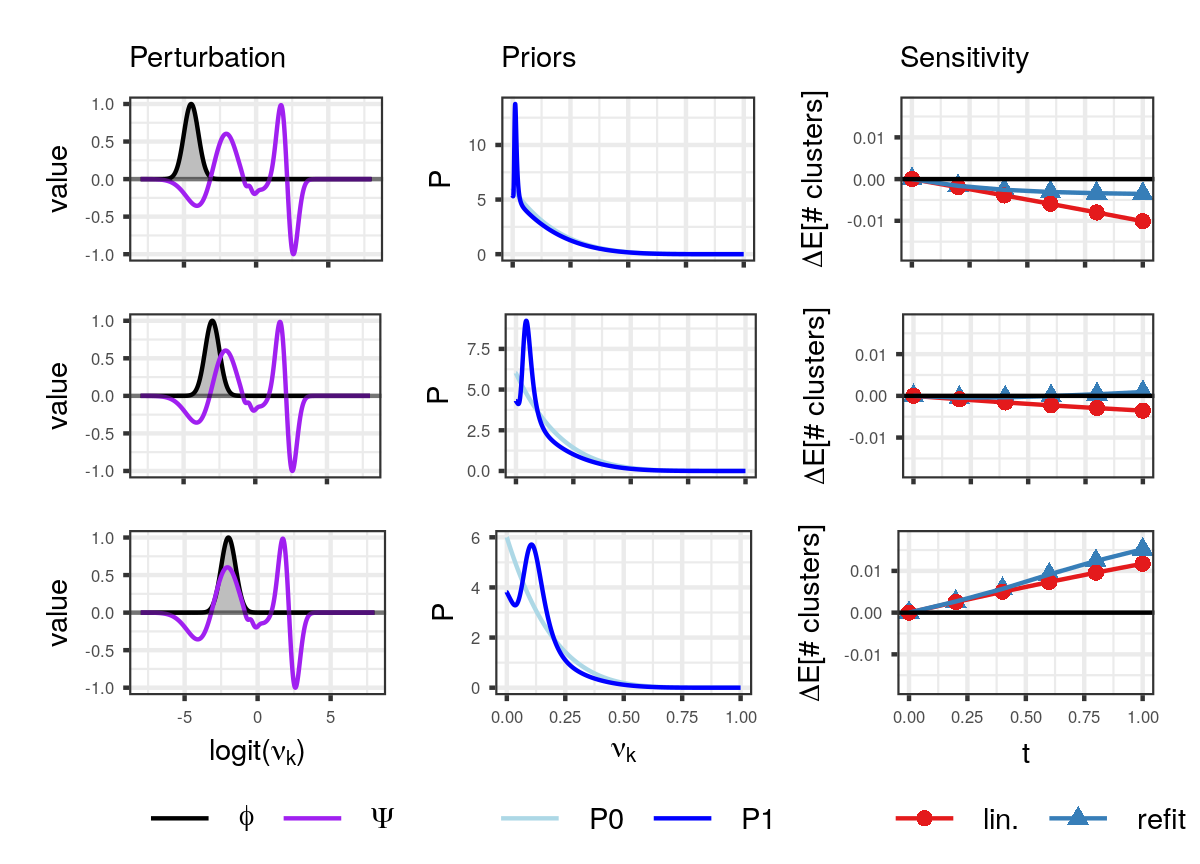
\includegraphics[width=0.784\linewidth,height=0.690\linewidth]{figure/iris_fpertall-1} 

}



\end{knitrout}
}


%%%%%%%%%%%%%%%%%%%%%%%
% iris worst-case
%%%%%%%%%%%%%%%%%%%%%%%%
\newcommand{\IrisWorstCase}{

\begin{knitrout}
\definecolor{shadecolor}{rgb}{0.969, 0.969, 0.969}\color{fgcolor}

{\centering 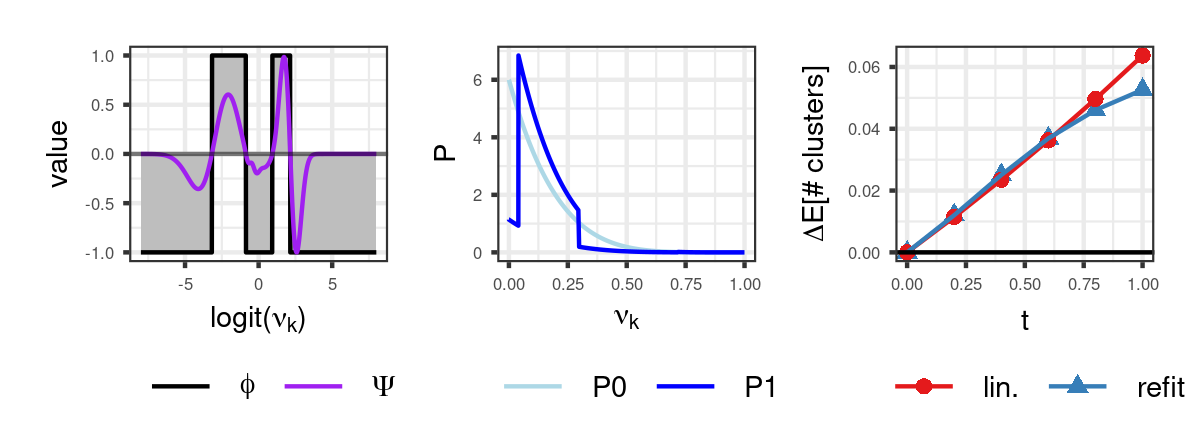
\includegraphics[width=0.784\linewidth,height=0.345\linewidth]{figure/iris_worstcase-1} 

}



\end{knitrout}
}

